\documentclass[10pt]{article}
\usepackage[a4paper,
            tmargin=3cm,
            bmargin=3cm,
            lmargin=2cm,
            rmargin=5.5cm,
            marginpar=3.5cm]{geometry}

% Don't necessarily need all of these, I just copied from my standard LaTeX config
\usepackage{parskip}
\usepackage{graphicx}
\usepackage{wrapfig}
\usepackage[hidelinks]{hyperref}
\usepackage{multirow}
\usepackage{array}
\usepackage{booktabs}
\hbadness 10000 % suppresses underfull hbox errors which are common with marginpar
\usepackage{float}
\usepackage[labelfont=it]{caption}
\captionsetup{belowskip=-0.4cm}
\newcommand{\figref}[1]{\textit{Figure \ref{fig:#1}}}
\usepackage{enumitem}
\usepackage{cmap}
\usepackage[scaled=0.8]{beramono} % This is nice because the tilde isn't at the top of the line.
\usepackage[T1]{fontenc}

\usepackage{tcolorbox}
\tcbuselibrary{listings}
\lstdefinestyle{tcbscript}{language={},
     belowskip=2pt, aboveskip=2pt,
     columns=fullflexible, keepspaces=true,
     breaklines=true, breakatwhitespace=true,
     basicstyle=\ttfamily\small, extendedchars=true, nolol
     }
\newtcblisting{script}[1]{
    title=#1,
    fontupper=\ttfamily,
    fonttitle=\bfseries,
    colframe=blue!60!gray,
    colback=blue!5,
    width=0.95\textwidth,
    center,
    listing only,
    listing style=tcbscript,
    beforeafter skip=0.45cm
}
\newtcblisting{cmdline}{
    fontupper=\ttfamily,
    colframe=white, opacityframe=0, % transparent
    colback=white, opacityback=0, % transparent
    width=0.95\textwidth,
    center,
    listing only,
    listing style=tcbscript,
    beforeafter skip=-0.05cm
}
\newtcolorbox{summary}[0]{
    center,
    width=0.95\textwidth,
    colback=red!5!white,
    colframe=red!75!black,
    fonttitle=\bfseries,
    title=Summary,
    beforeafter skip=0.45cm
}

\usepackage{amsmath}
\usepackage{amssymb}
\usepackage[version=4]{mhchem}
\usepackage{chemmacros}
\usepackage{siunitx}
\usepackage{upgreek}

% Bibliography
% \usepackage[style=chem-acs,biblabel=dot,subentry]{biblatex}
% \addbibresource{bib_file.bib}
% uncomment if needed

\usepackage{fancyhdr}
 
\pagestyle{fancy}
\fancyhf{}
\rhead{SBM CDT 2020}
\lhead{Practical Computational Chemistry Module}
\cfoot{\thepage}
\begin{document}

\textbf{\LARGE Getting Started -- Day 1}

\vspace{0.2cm}

\begin{tabular}{ll} % alphabetical surname order... And Fernanda should go first!
    \textbf{Tutors:} & Fernanda Duarte (fernanda.duartegonzalez@chem.ox.ac.uk) \\
     & Jonathan Yong (jonathan.yong@chem.ox.ac.uk) \\
     & Tom Young (tom.young@balliol.ox.ac.uk)
\end{tabular}

\vspace{0.2cm}

Welcome! In this set of exercises you will gain some hands-on experience in connecting to a remote cluster, creating input files for the computational chemistry programme ORCA, and submitting the calculations to the cluster's job management system. \marginpar{\small We will not discuss the theory behind the calculations: if you are interested, a few suggestions for books can be found in the \textit{Other resources} section at the end of this handout.}

Before starting, please install \textbf{MobaXterm} (from the Software Centre), \textbf{Avogadro} (version 1.2.0 from \url{https://avogadro.cc/}; the version in the Software Centre, 1.1.1, is not sufficent). You will need both these programmes to complete the following exercises. We also recommend installing a plain text editor such as \textbf{Notepad++} (\url{https://notepad-plus-plus.org/}).

As we go along, there will be certain sections where you are asked to note down a value or to answer some questions. \textbf{You will need to submit a short writeup (approximately one page long) containing these at the end of the course.}

\section{Connecting to the cluster}

The cluster we will be using is part of the Advanced Research Computing (ARC) facilities at Oxford (\url{https://help.it.ox.ac.uk/arc/index}). We need to connect to it remotely (via SSH), a functionality which is provided by MobaXterm. When opening MobaXterm for the first time, you may encounter a Windows Firewall prompt: make sure that access over domain networks is allowed.

Click \textbf{Session} (not ``Session\textbf{s}''!) at the top-left corner, then \textbf{SSH}. \marginpar{\small You can skip this in subsequent sessions by using the \textit{Remote sessions} section in the MobaXterm start screen.} In the resulting popup window (\figref{ssh}), enter \texttt{arcus-b.arc.ox.ac.uk} in the \textit{Remote host} box, tick the \textit{Specify username} checkbox, and enter the username you were given. Leave the remainder of the settings unchanged.

\begin{figure}[H]
    \centering
    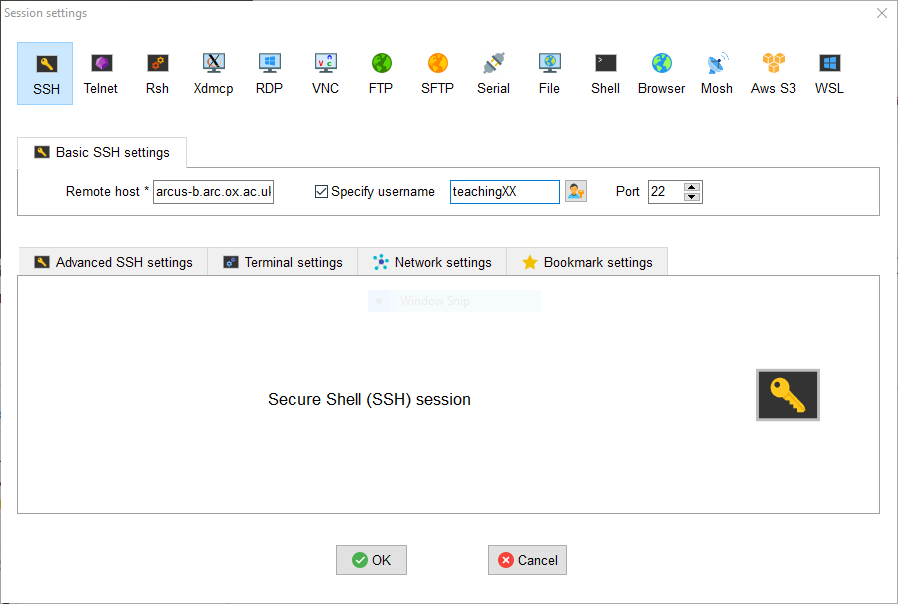
\includegraphics[scale=0.5]{./img/ssh}
    \caption{The SSH dialog in MobaXterm.}
    \label{fig:ssh}
\end{figure}\marginpar{\small When entering passwords into terminals, there is no visual feedback, so don't be alarmed.}

Click \textbf{OK}. Enter your password when prompted, then press Enter. You should be greeted with a terminal window on the right, and a graphical interface allowing you to browse files on the left (\figref{loggedin}):

\begin{figure}[H]
    \centering
    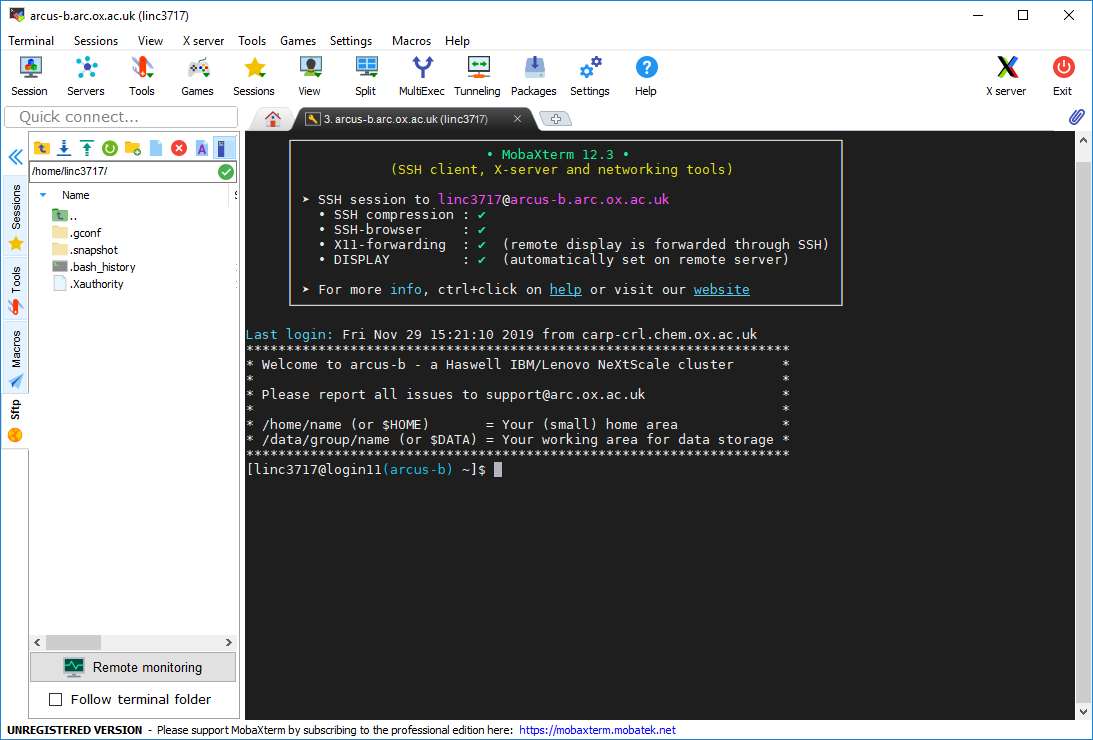
\includegraphics[scale=0.38]{./img/loggedin}
    \caption{The MobaXterm interface upon successfully logging in.}
    \label{fig:loggedin}
\end{figure}

\marginpar{\small Linux, MacOS, and Windows 10 systems have \textit{native} SSH capabilities, meaning that in principle you do not need to install any extra software to connect to a remote server. However, they do not provide the graphical interface in the left side of MobaXterm, so everything must be done exclusively from the terminal.}

Congratulations! You are now logged into the \texttt{arcus-b} cluster: it is from this screen that you will be able to submit calculations and monitor their output.

\section{Managing files on the cluster}

The left-hand pane in MobaXterm resembles the ``familiar'' File Explorer in Windows. Perhaps most importantly, it allows you to move files to and from the cluster in a drag-and-drop manner. You can try it with any file from your computer (but bear in mind that the file transfer can take a while depending on the file size).

Although this feature often comes in handy, it is also important to be (somewhat) comfortable with using the terminal. In this section we will go through several of the most basic commands for file and folder management. You may wish to skip ahead if you are already familiar with these.

The first thing that we notice is that the line you input text on is preceded by a series of characters (called a \textit{prompt}):

\begin{cmdline}
[username@hostname(arcus-b) ~]$
\end{cmdline}

The prompt contains some important information: your username, the hostname (the name of the computer you are connected to), and the current \textit{directory} you are in.\marginpar{\small The dollar sign \texttt{\$} has no particular meaning; it just happens to be one of the most commonly used characters for ending a prompt.} When you first log in, you will always find yourself in your \textit{home directory}, which is conventionally denoted by a tilde \texttt{\textasciitilde}. The command 

\begin{cmdline}
ls
\end{cmdline}

can be used to list the contents of the directory you are in. If you try that right now, you will probably get no output, because your home directory should be empty. We can populate it with a new (empty) folder by using:\marginpar{\small Notice how we use an underscore instead of a space in our file name. Spaces in file names are not prohi\-bited, but can potentially cause annoying problems which need to be carefully circumvented, so it is easier to avoid them altogether.}

\begin{cmdline}
mkdir cats
\end{cmdline}

and a new file with:

\begin{cmdline}
touch maine_coon.txt
\end{cmdline}

Now running \texttt{ls} should tell us that there are two things in the current directory, namely \texttt{cats} and \texttt{maine\_coon.txt} (try it!). This is not immediately reflected in the graphical browser; you will need to click on the \textit{Refresh} button (\figref{refresh}) to see them:

\begin{figure}[H]
    \centering
    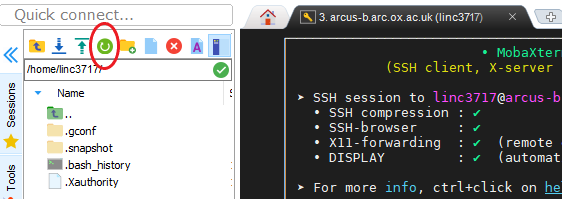
\includegraphics[scale=0.6]{./img/refresh}
    \caption{The Refresh button in MobaXterm's file browser.}
    \label{fig:refresh}
\end{figure}

We can now move \texttt{maine\_coon.txt} into the folder \texttt{cats}, either by dragging-and-dropping in the graphical interface, or by:\marginpar{\small Instead of \textit{moving} (\texttt{mv}) a file, you can also \textit{copy} it using \texttt{cp}. The syntax is the same: \texttt{cp <file> <destination>}.}

\begin{cmdline}
mv maine_coon.txt cats
\end{cmdline}

How do we check that the file was indeed moved? Just using \texttt{ls} now does not work, because \texttt{ls} only lists files in the current directory, which isn't \texttt{cats}. We need to change the current directory to \texttt{cats}:\marginpar{\small You can press Tab in the terminal to autocomplete file and folder names.}

\begin{cmdline}
cd cats
\end{cmdline}

After doing this, your prompt should change from \texttt{\textasciitilde} to \texttt{\textasciitilde /cats}: this indicates that you have successfully \textit{navigated} to the \texttt{cats} directory. Using \texttt{ls}, you can now verify that \texttt{maine\_coon.txt} is in this directory. To return to the previous directory, use:

\begin{cmdline}
cd ..
\end{cmdline}

The two dots \texttt{..} refer to the \textit{parent directory} of your current location. In this case, that would simply be your home directory, since \texttt{cats} was created inside your home directory.\marginpar{\small If you ever get hopelessly lost in the terminal, typing \texttt{cd} without any arguments will always bring you back to the safety of your home directory.}

To delete a folder you can use \texttt{rmdir}. If you are in your home directory, you can try to remove \texttt{cats} with:

\begin{cmdline}
rmdir cats
\end{cmdline}

but it will not work: the terminal will (helpfully) tell you that \texttt{cats} is not empty, so it refuses to delete it for you. We need to empty \texttt{cats} first before we can delete it. Navigate back inside there (\texttt{cd cats}) and delete the lone file there with:\marginpar{\small Unlike \texttt{rmdir}, the target of \texttt{rm} does not have to be empty for it to work. \textbf{BEWARE:} it is \textit{extremely} difficult to recover a file once you have \texttt{rm}'d it. It does not go to a Recycle Bin; it is simply \textit{gone}. So before running \texttt{rm} on something, make sure you really do want to delete it.}

\begin{cmdline}
rm maine_coon.txt
\end{cmdline}

Return to the parent directory (\texttt{cd ..}) and try to remove the \texttt{cats} directory again (\texttt{rmdir cats}). This time it should work, and if you type \texttt{ls} you will find that it is completely empty, as expected. In terms of the contents of your home directory, we are now back where we started, but hopefully this short journey will have shed some light on how the terminal works.

\begin{summary}
   \begin{itemize}[leftmargin=0.6cm]
        \item The prompt tells you useful stuff -- including your current directory.
        \item \texttt{ls}: lists all files and folders in the current directory.
        \item \texttt{mkdir}: creates empty directories.
        \item \texttt{touch}: creates empty files.
        \item \texttt{mv}: moves files.
        \item \texttt{cd}: changes your current directory.
        \item \texttt{rmdir}: removes empty directories.
        \item \texttt{rm}: removes files.
    \end{itemize}
\end{summary}

\section{Preparing an ORCA input file}

ORCA is a computational chemistry programme developed by the group of Frank Neese.\marginpar{\small "ORCA'' isn't actually an acronym: it just came about because Frank Neese went on a whale-watching cruise in California.} It takes an \textit{input file}, containing all the instructions for the calculation, and (after a while) returns an \textit{output file} containing all the results. ORCA can only be called using the terminal: there is no graphical interface, so you cannot (for example) draw a molecule in ChemDraw and click a button to run a calculation on it. In this section we will first analyse the structure of a simple input file, then look at how we can use molecular visualisation software such as Avogadro to help us generate input files.

A simple input file looks like the following:

\begin{script}{h2o\_bad\_geometry.inp}
! BP86 def2-SVP SP

*xyz 0 1
H -1.0 0.0 0.0
O  0.0 0.0 0.0
H  1.5 0.0 0.0
*
\end{script}

The first line

\begin{cmdline}
! BP86 def2-SVP SP
\end{cmdline}

is a \textit{keyword line}: it begins with a compulsory exclamation mark and contains several keywords which tell ORCA the level of theory as well as what type of calculation we want to do. In this case, \texttt{BP86} is a DFT functional, and \texttt{def2-SVP} a basis set. \texttt{SP} stands for \textit{single-point}, which refers to the simplest kind of calculation where we only want ORCA to tell you the energy of a molecule.\marginpar{\small Technically, the keyword \texttt{SP} is not needed: if you do not request a particular type of calculation, ORCA assumes you want a single-point. But it is a good idea to include it anyway, especially when starting out.}

The remainder of the input file tells ORCA what molecule you are interested in. In most computational chemistry software, molecules are not specified using connectivity information (i.e.\ what atom is bonded to what): instead, we specify the \textit{geometry} of the molecule, or in other words, the 3D position of each atom in the molecule. We need three coordinates \((x, y, z)\) to describe the position of one atom, and that is exactly what the three lines

\begin{cmdline}
H -1.0 0.0 0.0
O  0.0 0.0 0.0
H  1.5 0.0 0.0
\end{cmdline}

specify. For example, the first line tells ORCA that there is a hydrogen atom with the coordinates \((-1, 0, 0)\) (the units are angstroms: \(\SI{1}{\angstrom} = \SI{10e-10}{m})\). Pictorially, our molecule could be drawn as in \figref{h2obadgeom} below. Obviously, this is \textit{not} a realistic geometry for water: it should not be a linear molecule, and the \ce{O-H} bond distances should not be 1 and \SI{1.5}{\angstrom}! So, if we were to actually run this calculation, we should not be surprised to find that it is a rather unstable arrangement of atoms. When performing a single-point calculation, ORCA does not optimise the geometry of the molecule, and will just use whatever you give it.

It remains to explain the two lines surrounding the ``coordinate block''. The asterisks are there to signal the start and the end of the coordinates respectively.\marginpar{\small For another example, if you had a radical anion species, you would change the line to \texttt{*xyz -1 2}.} \texttt{xyz} tells ORCA the format in which we are providing the coordinates, namely, as \((x, y, z)\)-coordinates. \texttt{0} and \texttt{1} are the \textit{charge} and \textit{multiplicity} of the molecule respectively. Since water is a closed-shell molecule, its overall spin $S$ is zero, and the multiplicity (defined by $2S + 1$) is one (a singlet state).

\begin{figure}[H]
    \centering
    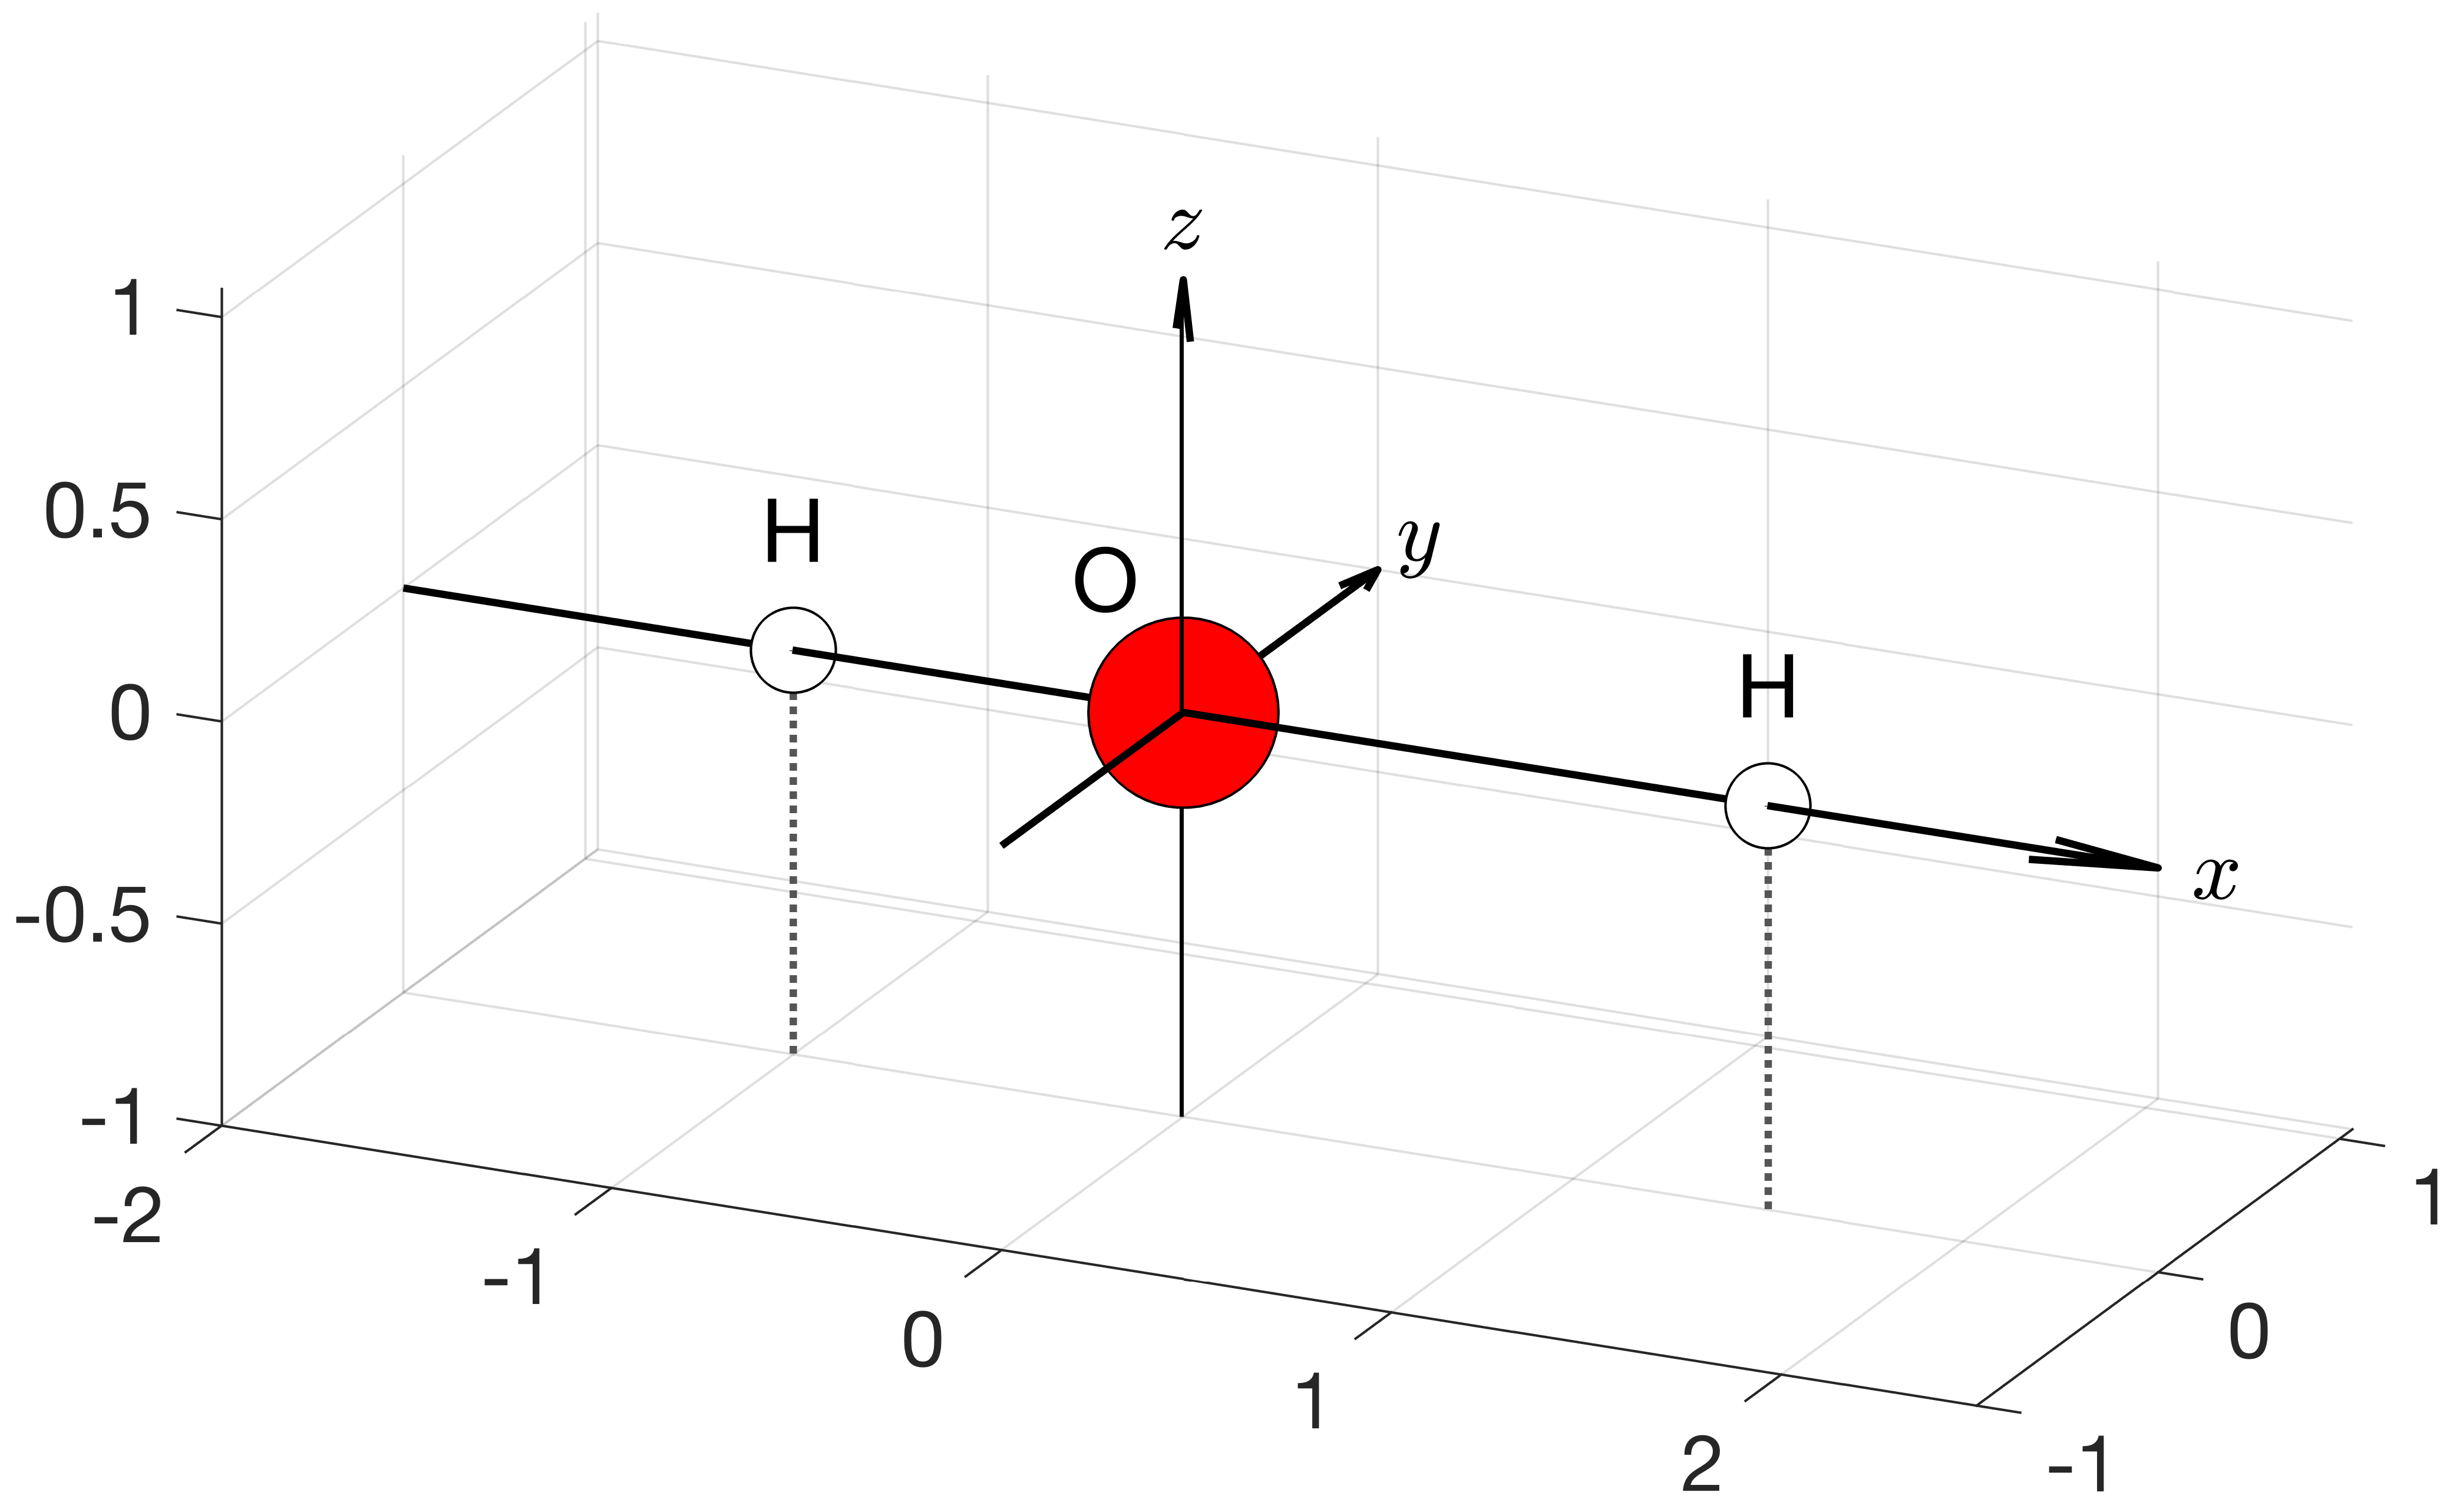
\includegraphics[scale=0.4]{./img/h2obadgeom}
    \caption{Our initial water geometry.}
    \label{fig:h2obadgeom}
    % I did this in MATLAB because I didn't want to faff around with pgfplots (also doing it in pgfplots would probably make compilation painfully slow). For reproducibility's sake, the MATLAB code is at the bottom of this document (after \end{document}). (Jon Y)
\end{figure}

If we want to obtain a more realistic value for the energy of a water molecule, we need to first \textit{optimise} the molecular geometry. That is to say, we need to instruct ORCA to find the minimum-energy geometry, and \textit{then} calculate the energy of water at that minimum-energy geometry. This can be done by simply replacing the \texttt{SP} keyword with \texttt{Opt}, for optimisation. With this keyword, ORCA will take your initial geometry and try to tweak it a little bit at a time until it reaches a minimum energy.

Bear in mind that to get a sensible optimised geometry, the initial geometry that you give ORCA has to be at least somewhat reasonable.\marginpar{\small The better your initial geometry, the faster the optimisation will be, too.} Our linear geometry is, unfortunately, not quite reasonable enough. But since we are dealing with water, the input file is relatively easy to construct by hand, and we could probably come up with a more sensible starting geometry without thinking too hard. What if, however, we wanted to look at larger, more interesting molecules? Enter Avogadro. 

When you first open Avogadro, you will see a blank canvas on which you can ``draw'' a molecule. The drawing interface is fairly intuitive; feel free to play around with it a little.\marginpar{\small You can rotate the camera angle by holding down the middle mouse button, pan by holding down the right mouse button, and right-click on atoms to delete them if you make a mistake.} Once you've drawn something, head over to the \textbf{Auto Optimisation Tool} (\figref{avoopt}):

\begin{figure}[H]
    \centering
    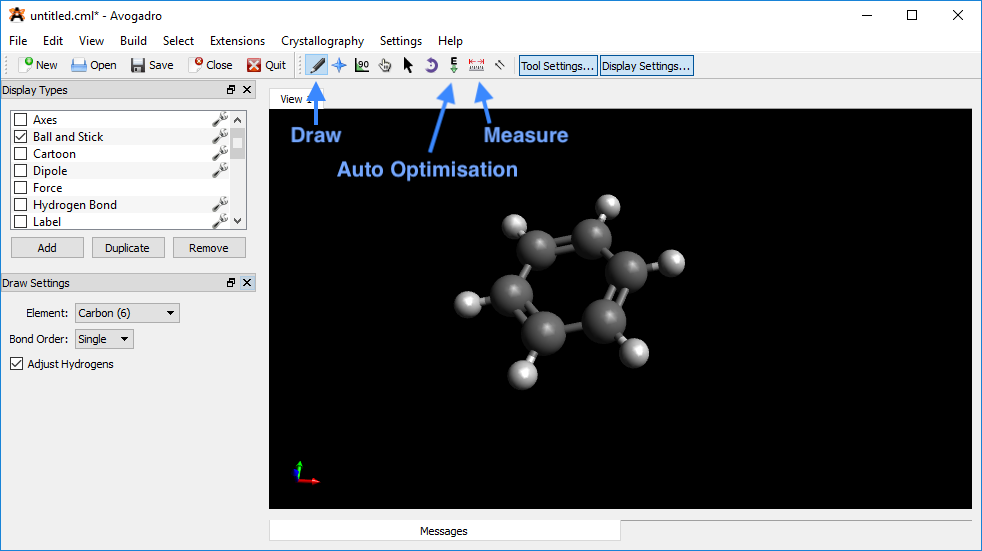
\includegraphics[scale=0.45]{./img/avoopt}
    \caption{The various tools available in Avogadro.}
    \label{fig:avoopt}
\end{figure} \marginpar{\small This optimisation is performed using a \textit{force field}, which represents a very low level of theory: it is good enough to generate initial geometries for the high-level ORCA calculations, but it is not quite accurate enough to draw serious conclusions from (or to publish!).}

Press the \textbf{Start} button, and Avogadro will perform a quick optimisation of your molecular geometry. Once the molecular geometry no longer changes, stop the optimisation and select (from the top) \textbf{Build > Cartesian Editor...} where you will find that Avogadro has prepared the entire coordinate block for us in the correct format! All that remains is to copy and paste the coordinate block into the ORCA input file and add the other lines detailing the level of theory and so on.

\begin{summary}
    \begin{itemize}[leftmargin=0.6cm]
        \item ORCA input files minimally consist of a \textit{keyword line} and a \textit{coordinate block}. The charge and multiplicity must also be specified.
        \item Coordinates are specified as \((x, y, z)\)-coordinates in angstroms.
        \item You can use Avogadro to generate coordinate blocks for use with ORCA.
    \end{itemize}
\end{summary}


\section{Submitting jobs to the cluster}

To run a calculation, we first need to get an input file onto the cluster. There are two main ways to do this. The first is to prepare the input file on your own computer, then drag-and-drop it into the MobaXterm pane. \textbf{Make sure you use a plain text editor, such as Notepad++, to prepare input files.} Programmes like Microsoft Word will not work as they add extra information about text formatting and layout.\marginpar{\small There is a third way, which is to use terminal-based text editors such as \texttt{vim}, \texttt{nano}, or \texttt{emacs}. Although these are powerful tools, they also come with a steep initial learning curve.}

\begin{figure}[H]
    \centering
    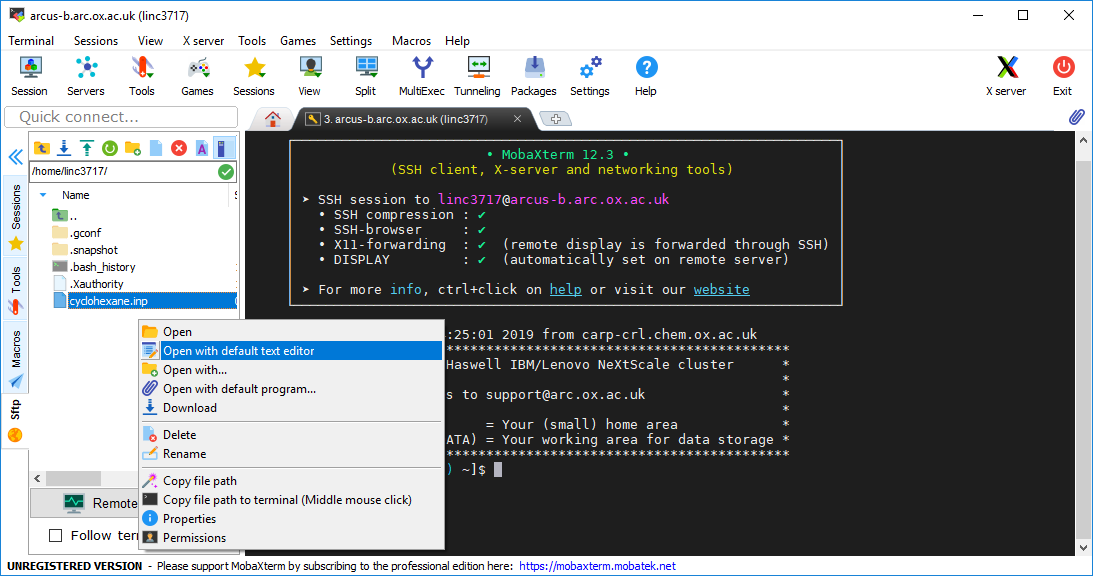
\includegraphics[scale=0.4]{./img/texteditor}
    \caption{Accessing the default text editor in MobaXterm.}
    \label{fig:texteditor}
\end{figure}

Alternatively, you can edit files on the cluster using the text editor built into MobaXterm. Once you have a file on the cluster (either by creating it from the terminal using \texttt{touch}, or by dragging-and-dropping), you can right-click it in the MobaXterm browser and select \textbf{Open with default text editor} (\figref{texteditor}).

Your first exercise will be to calculate the energy of cyclohexane, using the geometry pre-optimised by Avogadro. We will stick with the same level of theory as before, namely \texttt{BP86} and \texttt{def2-SVP}, as this is capable of reaching ``chemical accuracy'' while also being relatively computationally cheap. Your input file will look somewhat like the snippet below. We have suggested the name \texttt{c6h12\_sp.inp}, but you can give it any name you like, as long as you start with a letter and end with the file extension \texttt{.inp}.

\begin{script}{c6h12\_sp.inp}
! BP86 def2-SVP SP

%pal nprocs 16 end

*xyz 0 1
 ... (insert coordinates from Avogadro here) ...
*
\end{script}

The new line

\begin{cmdline}
%pal nprocs 16 end
\end{cmdline}

tells ORCA to use 16 CPU cores for the computation\marginpar{\small All computations on the \texttt{arcus-b} cluster are automatically allocated at least 16 CPUs, so it would be a waste to not make full use of it!} (which will speed it up significantly), and so we will use it henceforth.

To run a calculation, we need to submit it to the job scheduling software that manages the cluster. This requires a script, which you can obtain by running the following command in your terminal. Note that pasting text into the terminal (this particular one in MobaXterm, at least) is done using a right-click, not Ctrl-V. 

\begin{cmdline}
source <(wget -O - https://raw.github.com/duartegroup/sbmcc/master/cc20.sh)
\end{cmdline}

This will give you a new file called \texttt{qorca} in your home directory. It should be noted that \texttt{qorca} is not actually the ORCA programme itself; it merely requests the cluster to run the ORCA job using your input file. \marginpar{\small You \textit{must} do this in the terminal. MobaXterm's graphical file browser is not capable of submitting jobs.} To submit the input file you prepared earlier, first \texttt{cd} to the directory containing it, then run:

\begin{cmdline}
qorca c6h12_sp.inp
\end{cmdline}

You should see a confirmatory message that your job has been submitted. To check the progress of your job, you can use either:

\begin{cmdline}
squeue -u <username>
\end{cmdline}

which will print a list of your running jobs with their status (\texttt{PD} = pending and \texttt{R} = currently running). Once a job is complete, it will no longer show up. Alternatively, you can track the progress of the job using:

\begin{cmdline}
tail c6h12_sp.out
\end{cmdline}

which prints the last few lines of the output file. Notice that we are using the \texttt{.out} extension here (which corresponds to the output file) instead of our original \texttt{.inp}. When it finishes a calculation, the output file will have something similar to the following, which you can observe using \texttt{tail}:\marginpar{\small If the job ends (no longer shows up when using \texttt{squeue}) but the file does not end with this line, please consult a demonstrator.}

\begin{cmdline}
              ****ORCA TERMINATED NORMALLY****
TOTAL RUN TIME: 0 days 0 hours 0 minutes 16 seconds 827 msec
\end{cmdline}

\vspace{-0.2cm}

\begin{summary}
    \begin{itemize}[leftmargin=0.6cm]
        \item Input files can be prepared on your own desktop (using e.g.\ Notepad++) or on the terminal (using MobaXterm's editor).
        \item You can submit jobs on the cluster from the terminal using the \texttt{qorca} script.
        \item Job progress can be monitored using either \texttt{squeue} or \texttt{tail}.
    \end{itemize}
\end{summary}

\section{Comparing cyclohexane geometries}

If your job ran successfully, the output file should contain in excess of 1000 lines. For a more complicated calculation, such as an optimisation (which you will do soon), this number can grow very rapidly! How do we pick out the important information from all of that text?

One way is to manually inspect the file and look for certain keywords, which we will do now. Open up the output file \texttt{c6h12\_sp.out}, either by dragging it back to your desktop and using Notepad++, or by using the built-in MobaXterm editor. Look for a line near the end that reads \texttt{FINAL SINGLE POINT ENERGY}: this is the energy of your molecule in that particular geometry. Take note of this number.

Alternatively, we can use software to help us parse the output file. Avogadro is capable of doing this (to some extent). If you haven't already done so, copy your output file back to your own computer, then open it with Avogadro. It will display the final geometry from the ORCA calculation. Since this was a single-point calculation, ORCA does not change the geometry, so it will be exactly the same as the geometry you submitted. Use the \textbf{Measure Tool} (\figref{avoopt}) to measure some of the key properties listed below:\marginpar{\small We already learnt that bond lengths are specified in angstroms. You should now do some research to find out what the units of energy in computational chemistry are, and how they relate to familiar units such as kcal/mol or kJ/mol.}

\begin{itemize}
    \item \ce{C-C} and \ce{C-H} bond lengths (for both equatorial and axial protons)
    \item \ce{C-C-C} and \ce{H-C-H} bond angles
\end{itemize}

Once you have recorded these somewhere, make another copy of your input file, but change the \texttt{SP} keyword to \texttt{Opt}. This tells ORCA that we want to optimise the geometry. Submit this job (the calculation itself should not take more than 2 minutes) and analyse the output using the same steps as before. This time, when you open the output file, Avogadro will display the geometry as optimised by ORCA, which will be different from the previous geometry. Compare the energies, bond lengths, and bond angles obtained from the two calculations. How different are they?

\begin{summary}
    \begin{itemize}[leftmargin=0.6cm]
        \item Single-point calculations involve ORCA calculating the energy of one single given geometry, whereas optimisations allow ORCA to search for a minimum-energy geometry.
        \item Simple pieces of information such as energies can be obtained by visual inspection of ORCA output files.
        \item Avogadro is useful for visualising final geometries.
    \end{itemize}
\end{summary}


\section{Conformational analysis}

In this next exercise we will study an \(\alpha\)-halocarbonyl compound. Our prototype molecule is (\textit{S})-2-fluoropropanal, for which the starting geometry can be downloaded from \url{https://raw.githubusercontent.com/duartegroup/sbmcc/master/s2fp.xyz}. Open up the \texttt{.xyz} file with a text editor. You should find that it contains the desired coordinate block, along with two more lines at the top. The first line (\texttt{10}) is the number of atoms in the molecule, and the second line is a comment line which can be anything. This is the standard format for \texttt{.xyz} files.

We will first look at how the energy of the molecule varies with the \ce{O-C-C-F} dihedral angle. To do this, we need to do a series of optimisations where the dihedral angle is constrained to a particular value.\marginpar{\small If we did not constrain the dihedral angle, it would simply be optimised to a (local) minimum, and we would not learn anything about the rest of the PES.} This is called a \textit{potential energy surface} (PES) \textit{scan}, and can be performed by invoking an additional \texttt{Scan} line. For this exercise, we will use Hartree--Fock theory instead of DFT to speed up the calculations, so we replace the original \texttt{BP86 def2-SVP} with \texttt{HF-3c}.

\begin{script}{s2fp\_scan.inp}
! HF-3c Opt

%pal nprocs 16 end

%geom Scan <SCAN_COORDINATES> end end

*xyz 0 1
 ... (paste the coordinates from the .xyz file in here) ...
*
\end{script}

We still need to specify the coordinate that we are scanning over. In this case, it is a dihedral angle, and in ORCA this is specified using the syntax

\begin{cmdline}
D <atom1> <atom2> <atom3> <atom4> = <initial>, <final>, <number_of_steps>
\end{cmdline}

We can set the initial value to 60, the final value to 420, and the number of steps to 19.\marginpar{\small \(420^\circ\) is the same as \(60^\circ\), of course, and using 19 steps means we get precisely a \(20^\circ\) difference between each step. Why start at \(60^\circ\) instead of \(0^\circ\)? It turns out that our initial geometry has this dihedral angle close to \(60^\circ\), and it's always better to start a scan from a value that is close to the initial geometry.} Now we just need to specify which atoms form the dihedral angle of interest. In ORCA this is done using the \textit{atom number}: the first atom listed in the coordinate block has number 0, the second atom has number 1, and so on. The fastest way of finding the atom numbers is to use software such as Avogadro.

\begin{figure}[H]
    \centering
    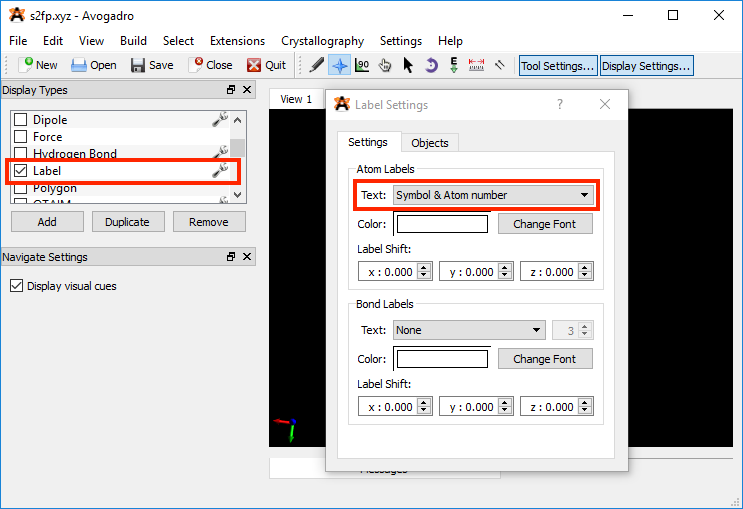
\includegraphics[scale=0.5]{./img/avolabel}
    \caption{Enabling atom labels in Avogadro.}
    \label{fig:avolabel}
\end{figure}

Open up the \texttt{.xyz} file you downloaded earlier with Avogadro. In the left-hand \textbf{Display Types} pane, scroll down to \textbf{Label} and make sure the checkbox next to it is ticked (\figref{avolabel}). Then, click the spanner on the right. This will bring up a settings pane.\marginpar{\small If the \textbf{Display Types} pane is not visible, click on \textbf{Display Settings...} at the top-right corner to open it.} Under \textbf{Atom Labels > Text}, select \textbf{Symbol \& Atom number}. Close the settings pane and you should now see that each atom in the molecule is labelled with the element symbol as well as the atom number.

\textbf{There is a catch: atom numbers in Avogadro start from 1, whereas ORCA starts from 0.} So, whenever you are preparing an ORCA input file, always remember to subtract 1 from the number Avogadro shows. Find the atom numbers that we are interested in: these are respectively the carbonyl oxygen, carbonyl carbon, $\alpha$-carbon, and fluorine. Substitute these into the input file to get:\marginpar{\small The order in which you specify the numbers matters! Any other combination will specify a \textit{different} dihedral angle from what we want. You can reverse them (\texttt{D 6 1 0 8 = ...}), but the corresponding dihedral angle will have the opposite sign, so you should start the scan from \(-60^\circ\).}

\begin{script}{s2fp\_scan.inp}
! HF-3c Opt

%pal nprocs 16 end

%geom Scan D 8 0 1 6 = 60, 420, 19 end end

*xyz 0 1
 ... (paste the coordinates from the .xyz file in here) ...
*
\end{script}

Submit the job on the cluster as before. This calculation should take just under 10 minutes. When it is complete, open up the \texttt{.out} output file and search for the text

\begin{cmdline}
The Calculated Surface using the 'Actual Energy'
\end{cmdline}

Under this line there are two columns of numbers:\marginpar{\small There is also a surface using the "SCF energy", but this neglects other contributions such as dispersion.} unsurprisingly, these are respectively the value of the dihedral angle, and the energy. Use a programme of choice to plot a graph of energy against the dihedral angle (it is a good idea to first convert the energies to more understandable units). You should find that there are two minima in the resulting graph, which represent the two conformers. Answer the following questions:

\begin{itemize}
    \item What are the relative populations of the two conformers at \SI{298}{K}? Use the Boltzmann distribution:\marginpar{\small In principle, these should be calculated using Gibbs free energies, not pure electronic energies as we are doing here.}
        \[ \frac{p_i}{p_j} = \exp\left(-\frac{\varepsilon_i - \varepsilon_j}{k_\mathrm{B}T}\right) \]
    \item What is the activation barrier for the conversion of the low-energy conformer to the high-energy conformer? What is the corresponding rate at \SI{298}{K}? Use the Eyring equation (assume the transmission coefficient \(\kappa = 1\)):
        \[ k = \frac{\kappa k_\mathrm{B}T}{h} \exp\left(-\frac{\Delta E}{k_\mathrm{B}T}\right) \]
    \item Qualitatively, how might you expect your results to change if we included solvation by a polar solvent such as DMSO? (If you have spare time and would like to run this calculation, consult a demonstrator.)
\end{itemize}

If you wish to inspect the optimised geometries, ORCA also outputs \texttt{.xyz} files for each step of the scan. For example, \texttt{<filename>.001.xyz} corresponds to the first step of the scan (which has the dihedral angle set to \(60^\circ\)), and so on.

\begin{summary}
    \begin{itemize}[leftmargin=0.6cm]
        \item \texttt{.xyz} files consist of two lines, plus the coordinate block used for ORCA input files.
        \item Atom labels start from 0 in ORCA, but start from 1 in Avogadro.
        \item In a PES scan, ORCA calculates how the energy of a system changes as one or more parameters are varied.
    \end{itemize}
\end{summary}



\section{Finding a transition state}

In the previous section we introduced the concept of a PES scan. By judicious choice of the parameter(s) being scanned over, it is possible to use this to study the course of a chemical reaction. The \textit{reaction coordinate} of a simple reaction can be characterised by one single parameter, such as a bond length or a bond angle. Here we will study the intramolecular tautomerisation of malonaldehyde (\figref{taut}):

\begin{figure}[H]
    \centering
    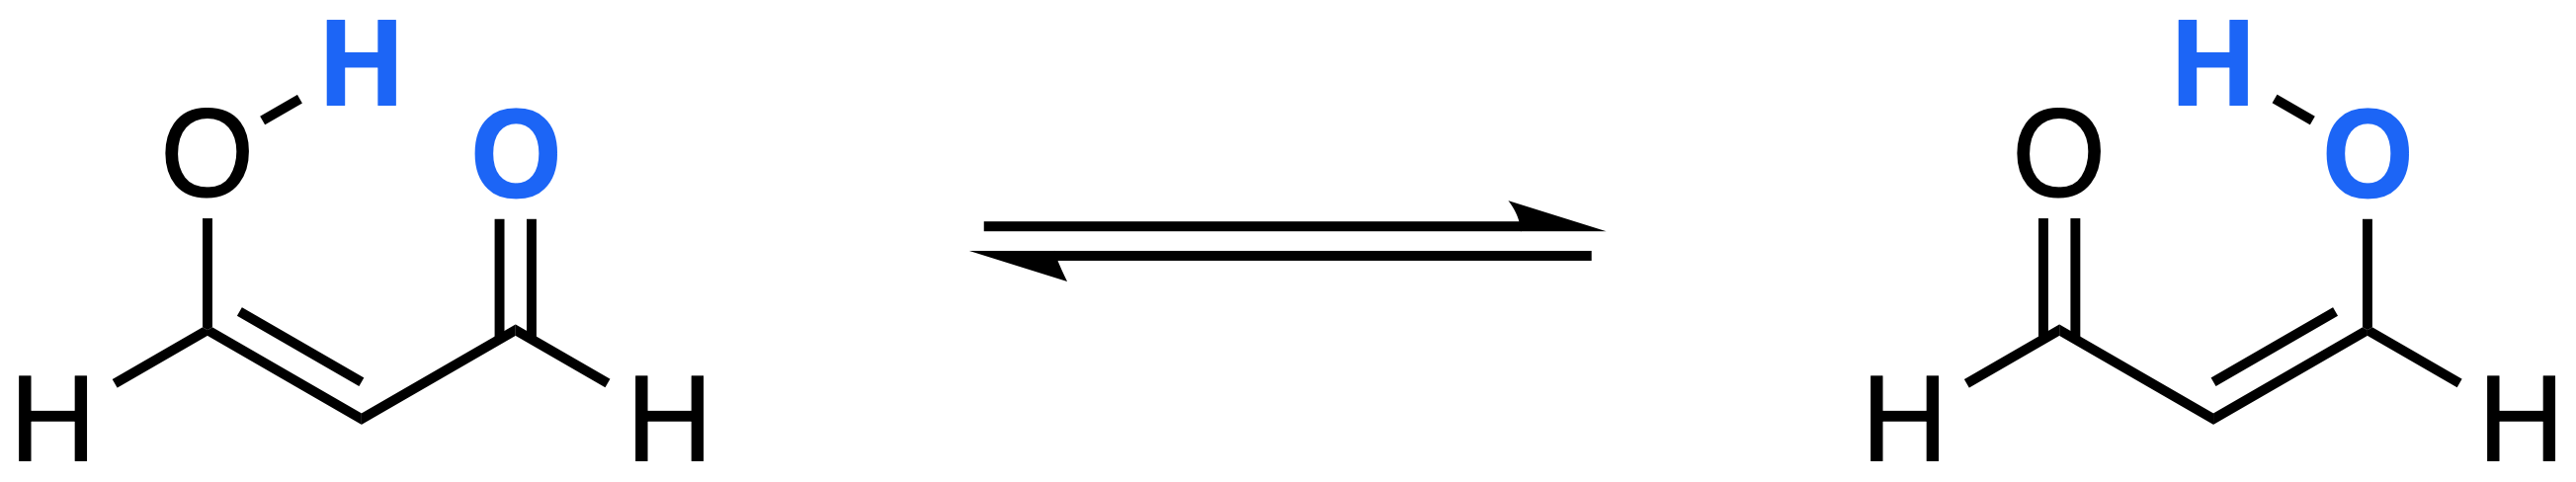
\includegraphics[scale=0.8]{./img/taut}
    \caption{Intramolecular tautomerisation of malonaldehyde.}
    \label{fig:taut}
\end{figure}

As the tautomerisation proceeds (from reactant to product), the distance between the highlighted oxygen and hydrogen atoms smoothly decreases. So, we can perform a bond length scan. The syntax is similar to the dihedral angle scan we did previously. You can obtain the initial geometry (already pre-optimised with \texttt{BP86/def2-SVP}) from \url{https://raw.githubusercontent.com/duartegroup/sbmcc/master/malon.xyz}.

Our starting ``bond length'' (it isn't really a bond yet) is the internuclear separation in the initial geometry, which should be \(\sim \SI{1.48}{\angstrom}\). The final bond length can be determined from an optimised geometry of the product -- which, in this case, is exactly the same as the reactant -- so we can measure the final bond length as being \(\sim \SI{1.06}{\angstrom}\). We will use 12 steps, and \texttt{BP86/def2-SVP} as the level of theory. Your input file should look like:

\begin{script}{malon\_scan.inp}
! BP86 def2-SVP Opt

%pal nprocs 16 end

%geom Scan B 8 4 = 1.48, 1.06, 12 end end

*xyz 0 1
 ... (paste coordinates here) ...
*
\end{script}

(Notice we use \texttt{B} for bond length, instead of \texttt{D}, inside the \texttt{Scan} line.) Submit this input file: it should take around 5 minutes to run. Once it is complete, plot the potential energy surface in the same way as before.

You should find that somewhere in the middle, there is a maximum in the energy. Find the \texttt{.xyz} file which corresponds to this maximum (don't forget that our scan was in decreasing order of bond length, so \texttt{.001.xyz} corresponds to the largest distance). This represents a geometry that is very close to the transition state.\marginpar{\small It is not \textit{exactly} the transition state, because the surface is not smooth: we only used discrete values of the bond length.} We will now use that geometry as a starting guess for a transition state search. Before proceeding, make a note of the key \ce{O-H} distances in this structure. 

For a transition state search, there are several changes to make to the input file:

\begin{itemize}
    \item The \texttt{OptTS} keyword requests an optimisation to a transition state (instead of \texttt{Opt}, which optimises to a minimum);
    \item We also add the \texttt{Freq} keyword which requests vibrational frequencies. This is very important for characterising transition states, which should have one (and only one) imaginary frequency;\marginpar{\small The imaginary frequency is related to the fact that a transition state is a maximum along only one direction, which is the reaction coordinate. Maxima are associated with a negative force constant, and the corresponding frequency is proportional to the square root of the force constant.}
    \item Since we are not doing a scan any more, we can remove the \texttt{Scan} line;
    \item In place of it, we add a line (\texttt{Calc\_Hess}) which instructs ORCA to calculate a Hessian before beginning the optimisation: this helps to guide the optimisation and makes it much more likely to succeed.
\end{itemize}

All in all, this gives us:

\begin{script}{malon\_ts.inp}
! BP86 def2-SVP OptTS Freq

%pal nprocs 16 end

%geom Calc_Hess true end

*xyz 0 1
 ... (paste coordinates here from .00X.xyz file) ...
*
\end{script}

This calculation should take under a minute. Open up the optimised transition state geometry with Avogadro and compare the \ce{O-H} bond lengths with the bond lengths you noted down previously. How different are they? Which geometry is more symmetric, and is that in line with what you expect based on the symmetry of the system under investigation?

As the final part of this tutorial, we will look at the vibrational modes of the transition state you have found. Search for the section containing \texttt{VIBRATIONAL FREQUENCIES}. You should find that the first six ``vibrational'' frequencies are zero.\marginpar{\small The zero-frequency ``vibrations'' are actually translations and rotations.} These are followed by one \textit{negative} frequency, which is (unfortunately) the conventional way of representing \textit{imaginary} frequencies. The rest of the frequencies should be positive.

We need to visualise this imaginary mode to make sure that it is indeed the vibrational mode that we are interested in -- namely the reaction coordinate. To do this, we use an ORCA helper utility called \texttt{orca\_pltvib}: this is capable of reading the \texttt{.hess} file which should have been produced by the TS calculation. Run the following two commands:

\begin{cmdline}
module load orca/4.2.0
orca_pltvib malon_ts.hess 6
\end{cmdline}

(Don't use the \texttt{.001.hess} file -- that is the \textit{initial} Hessian which we told ORCA to calculate using \texttt{Calc\_Hess}.)\marginpar{\small If you're wondering what a Hessian is: it's a matrix containing all the second derivatives of energy with respect to nuclear positions.} The number \texttt{6} refers to the imaginary frequency (remember ORCA counts from 0, so the numbers 0 through 5 correspond to the zero-frequency modes). Once you have done this, there should be a new \texttt{.hess.v006.xyz} file in the directory. Open it in Avogadro and select \textbf{Extensions > Animation...}. We recommend ticking both \textbf{Dynamic Bonds} and \textbf{Loop}. When you press the Play button, you should see that the imaginary mode does indeed correspond to the reaction coordinate, which brings reactant to product via the transition state we found.

\begin{summary}
    \begin{itemize}[leftmargin=0.6cm]
        \item The maximum in a PES scan can be used as a starting geometry for a transition state search.
        \item Transition states are characterised by one imaginary frequency.
        \item Vibrational modes can be visualised using \texttt{orca\_pltvib}.
    \end{itemize}
\end{summary}

\section{Other resources}

\textbf{Books}

\begin{itemize}
    \item J. Harvey, {\it Computational Chemistry}. Oxford Chemistry Primers, 2018. ISBN: 9780198755500.
    \item S. Bachrach, {\it Computational Organic Chemistry (2$^{nd}$ Edition)}. John Wiley \& Sons, 2004. ISBN 9781118291924.
    \item C. J. Cramer, {\it Essentials of Computational Chemistry (2$^{nd}$ Edition)}. John Wiley \& Sons, 2004. ISBN: 978-0-470-09182-1.
    \item F. Jensen {\it Introduction to Computational Chemistry (2/3$^{rd}$ Edition)}. John Wiley \& Sons. ISBN: 978-1-118-82599-0.
    \item H. P. Hratchian and H. B. Schlegel, Chapter 10 - Finding minima, transition states, and following reaction pathways on {\it ab initio} potential energy surfaces (pg 195-249) in {\it Theory and Applications of Computational Chemistry}. link: \url{ http://www.pitt.edu/~jordan/chem3430/289.TACC.pdf}
\end{itemize}

\textbf{Websites}

\begin{itemize}
    \item Anna Tomberg -- \url{https://www.youtube.com/user/IaNuisha} (search for Avogadro / ORCA videos) 
    \item ORCA manual and forums -- \url{https://orcaforum.kofo.mpg.de/} (need to register first)
    \item ORCA Input Library -- \url{https://sites.google.com/site/orcainputlibrary/} 
\end{itemize}

\newpage

\textbf{\LARGE Projects -- Day 2}

\begin{itemize}
   \item We will split the class into three groups of four people each. Choose whom you wish to work with.
    \item Choose one of the topics shown below. For each of them, there is an associated paper which you will do practical work on. 
    \item Read the paper (experimental \& computational data) before Day 2 starts. You will be tasked with investigating the scientific problem at hand, using the authors' work as a reference; you can also explore any other novel aspects which you may find relevant.
    \item Each group will have to prepare a (15 + 5) minute presentation for the last day.  The presentation should include background about the paper; the rationale behind the technique used; and analysis of the most relevant computational results which your group obtained. Any novel aspect explored will be a plus.
\end{itemize}

\section*{Projects}


\begin{enumerate}
    \item \href{https://doi.org/10.1038/s41557-018-0079-7}{\textcolor{blue}{Concerted Nucleophilic Aromatic Substitutions}}

        E.\ E.\ Kwan, Y.\ Zeng, H.\ A.\ Besser, E.\ N.\ Jacobsen. \textit{Nat. Chem.} \textbf{2018,} \textit{10,} 917--923. DOI: 10.1038/s41557-018-0079-7.
 
          \textbf{Abstract}: Nucleophilic aromatic substitution (S\textsubscript{N}Ar) is one of the most widely applied reaction classes in pharmaceutical and chemical research, providing a broadly useful platform for the modification of aromatic ring scaffolds. The generally accepted mechanism for S\textsubscript{N}Ar reactions involves a two-step addition--elimination sequence via a discrete, non-aromatic Meisenheimer complex. Here we use \ce{^{12}C}/\ce{^{13}C} kinetic isotope effect (KIE) studies and computational analyses to provide evidence that prototypical S\textsubscript{N}Ar reactions in fact proceed through concerted mechanisms. The KIE measurements were made possible by a new technique that leverages the high sensitivity of \ce{^{19}F} as an NMR nucleus to quantitate the degree of isotopic fractionation. This sensitive technique permits the measurement of KIEs on 10 mg of natural abundance material in one overnight acquisition. As a result, it provides a practical tool for performing detailed mechanistic analyses of reactions that form or break C--F bonds.

          \textbf{Technique}: Density Functional Theory; \textbf{Software}: {ORCA}

          \vspace{0.5cm}

    \item \href{https://doi.org/10.1039/C6CC07875C}{\textcolor{blue}{A DFT Study of the Role of Water in the Rhodium-Catalyzed Hydrogenation of Acetone}}

        V.\ Polo, R.\ R.\ Schrock and L.\ A.\ Oro. \textit{Chem.\ Commun.} \textbf{2016,} \textit{52,} 13881--13884. DOI: 10.1039/C6CC07875C.
 
          \textbf{Abstract}:The positive effect of the addition of water to acetone hydrogenation by \ce{[RhH2(PR3)2S2]+} catalysts has been studied by DFT calculations. The studied energetic profiles reveal that the more favourable mechanistic path involves a hydride migration to the ketone followed by a reductive elimination that is assisted by two water molecules.

          \textbf{Technique}: Density Functional Theory;  \textbf{Software}: {ORCA}

          \vspace{0.5cm}

    \item \href{https://doi.org/10.1021/acs.orglett.6b02341}{\textcolor{blue}{Structure Revision of an Acorane Sesquiterpene Cordycepol A}}

        D.\ S.\ Reddy, A.\ G.\ Kutateladze. \textit{Org.\ Lett.} \textbf{2016}, \textit{18,} 4860--4863.\\DOI: 10.1021/acs.orglett.6b02341.
 
          \textbf{Abstract}: Structure revision of a recently reported spirodecane sesquiterpene, cordycepol A, from fungi Cordyceps ophioglossoides was enabled by fast and accurate calculations of nuclear spin-spin coupling constants (SSCCs) with a relativistic force field (DU8c) parametric method. Two other reported cordycepols, B and C, are also identified as misassigned. Calculations of accurate SSCCs, which contain a wealth of structural information, offer a chemically intuitive tool for structure elucidation, rendering the whole structure revision process more guided and intentional, while augmenting in a synergistic way the calculations of chemical shifts.

          \textbf{Technique}: Density Functional Theory; \textbf{Software}: {ORCA}

          \vspace{0.5cm}
  
    \item \href{https://doi.org/10.1021/acscatal.5b01639}{\textcolor{blue}{Expanding the Catalytic Triad in Epoxide Hydrolases and Related Enzymes}}

        B.\ A.\ Amrein, P.\ Bauer, F.\ Duarte, A.\ J.\ Carlsson, A.\ Naworyta, S.\ L.\ Mowbray, M.\ Widersten and S.\ C.\ L.\ Kamerlin, \textit{ACS Catal.} \textbf{2015}, \textit{5,} 5702--5713. DOI: 10.1021/acscatal.5b01639.

        \textbf{Abstract}: Potato epoxide hydrolase 1 exhibits rich enantio- and regioselectivity in the hydrolysis of a broad range of substrates. The enzyme can be engineered to increase the yield of optically pure products as a result of changes in both enantio- and regioselectivity. It is thus highly attractive in biocatalysis, particularly for the generation of enantiopure fine chemicals and pharmaceuticals. The present work aims to establish the principles underlying the activity and selectivity of the enzyme through a combined computational, structural, and kinetic study using the substrate \textit{trans}-stilbene oxide as a model system. Extensive empirical valence bond simulations have been performed on the wild-type enzyme together with several experimentally characterized mutants. We are able to computationally reproduce the differences between the activities of different stereoisomers of the substrate and the effects of mutations of several active-site residues. In addition, our results indicate the involvement of a previously neglected residue, H104, which is electrostatically linked to the general base H300. We find that this residue, which is highly conserved in epoxide hydrolases and related hydrolytic enzymes, needs to be in its protonated form in order to provide charge balance in an otherwise negatively charged active site. Our data show that unless the active-site charge balance is correctly treated in simulations, it is not possible to generate a physically meaningful model for the enzyme that can accurately reproduce activity and selectivity trends. 

          \textbf{Technique}: Molecular Dynamics; \textbf{Software}: {Gromacs}

          \vspace{0.5cm}

    \item \href{https://doi.org/10.1021/ja068899t}{\textcolor{blue}{Carbene Stabilization by Aryl Substituents. Is Bigger Better?}}

        H.\ L.\ Woodcock, D.\ Moran, B.\ R.\ Brooks, P.\ v.\ R.\ Schleyer, H.\ F.\ Schaefer, \textit{J.\ Am.\ Chem.\ Soc.} \textbf{2007}, \textit{129,} 3763--3770. DOI: 10.1021/ja068899t.

          \textbf{Abstract}: The geometries and relative stabilities of the singlet and triplet states of phenyl- (\(C_\mathrm{s}\)), diphenyl- (\(C_2\)), 1-naphthyl- (\(C_\mathrm{s}\)), di(1-naphthyl)- (\(C_2\)), and 9-anthryl-substituted (\(C_\mathrm{s}\)) carbenes were investigated at the B3LYP/6-311+G(d,p) + ZPVE level of density functional theory. The singlet--triplet energy separations (\(\Delta E_\mathrm{ST}\)), 2.7, 2.9, 3.4, 3.7, and 5.7 kcal/mol, respectively, after including an empirical correction (2.8 kcal/mol) based on the error in the computed singlet--triplet gap for methylene versus experiment, are in good agreement with available experimental values. Consistent with literature reports, triplet di(9-anthryl)carbene has a linear, \(D_\mathrm{2d}\) symmetrical, allene structure with \SI{1.336}{\angstrom} C=C bond lengths and considerable biradical character. B3LYP favors such cumulene biradical structures and triplet spin states and predicts a large (>15 kcal/mol) “di(9-anthryl)carbene” singlet--triplet (biradical) energy gap. The resonance stabilization of both singlet and triplet carbenes increases modestly with the size of the arene substituent and overall, (di)arylcarbenes, both singlet and triplet, are better stabilized by bigger substituents. For example, methylene is stabilized more by a naphthyl than a phenyl group (singlets, 26.6 versus 24.4; and triplets, 20.9 versus 18.1 kcal/mol, respectively). The carbene geometries are affected by both steric effects and arene--carbene orbital interactions (\(\sigma\)--p and p--\(\pi\)). For instance, the central angles at the carbene are widened by a second arene group, which leads to increased s-character and shorter carbene bond lengths (i.e., \"{C}--C, \"{C}--H). In general, the aromaticity of the substituted rings in triplet carbenes is most affected by the presence of the unpaired electrons.

          \textbf{Technique}: Density Functional Theory; \textbf{Software}: ORCA

\end{enumerate}

\end{document}

% MATLAB code for the water geometry figure.
X = [-1; 0; 1.5];
Y = [0; 0; 0];
Z = [0; 0; 0];
sz = [300; 1500; 300];
color = [255 255 255; 255 0 0; 255 255 255];

scatter3(X, Y, Z, sz, color, 'filled', 'MarkerEdgeColor', 'k')
hold on
quiver3(0, 0, -1, 0, 0, 2.3, 'LineWidth', 1.5, 'Color', 'k')
quiver3(0, -1, 0, 0, 2.3, 0, 'LineWidth', 1.5, 'Color', 'k')
quiver3(-2, 0, 0, 5, 0, 0, 'LineWidth', 1.5, 'Color', 'k')
line([-1 -1], [0 0], [0 -1], 'LineWidth', 1.5, 'LineStyle', ':', 'Color', '#555555')
line([1.5 1.5], [0 0], [0 -1], 'LineWidth', 1.5, 'LineStyle', ':', 'Color', '#555555')
text(0, 0, 1.2, '$z$', 'Interpreter', 'latex', 'FontSize', 18, 'HorizontalAlignment', 'Center')
text(0, 1.3, 0, '$y$', 'Interpreter', 'latex', 'FontSize', 18, 'HorizontalAlignment', 'Center')
text(2.65, 0, 0, '$x$', 'Interpreter', 'latex', 'FontSize', 18, 'HorizontalAlignment', 'Center')
text(-1, 0, 0.3, 'H', 'FontSize', 18, 'HorizontalAlignment', 'Center')
text(-0.2, 0, 0.3, 'O', 'FontSize', 18, 'HorizontalAlignment', 'Center')
text(1.5, 0, 0.3, 'H', 'FontSize', 18, 'HorizontalAlignment', 'Center')
grid on
view([25 20])
axis equal
ax = gca;
ax.FontSize = 16;
print(gcf,'h2obadgeom.png','-dpng','-r600');
